\documentclass{article}
\usepackage{parskip}
\usepackage{graphicx}
\graphicspath{ {./images/} }

\title{CQS: Command Query Separation}
\author{Andreas Wenzelhuemer}

\begin{document}

\maketitle

The topic of this pattern will be about the architectural pattern called Command Query Separation (CQS).
CQS splits the backend of an application in two areas, in queries and commands (see figure~\ref{fig:cqs}).

\begin{figure}
    \centering
    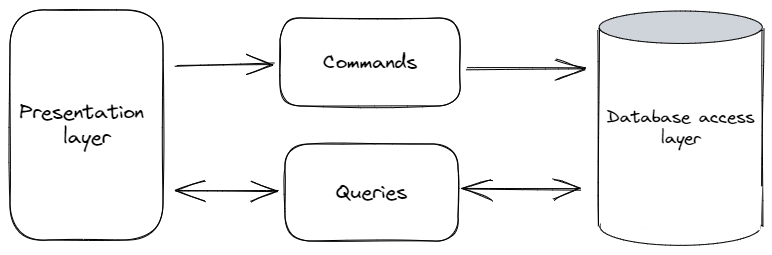
\includegraphics[width=0.7\textwidth]{images/CQS.png}
    \caption{CQS}
    \label{fig:cqs}
\end{figure}

\begin{itemize}
    \item {Queries: Are responsible for returning the right values, but never modify anything (there are no side effects).}
    \item {Commands: They change the state of the system but do not return any values.}
\end{itemize}

There exist multiple different implementations, but normally there is one object one for representing the operation and a handler class, which contains the actual implementation.
A so called dispatcher object is responsible for passing the given request to the correct handler.
Additionally here is also an extension of the pattern, the so called Command Query Responsibility Segregation (CQRS).
In this pattern, updates and reads are performed on separate databases and the read database gets synchronized when the data in the other database gets updated.

So the paper will contain following:
\begin{itemize}
    \item {CQS: What is it and how to use it.}
    \item {CQRS: What's the difference between CQS and CQRS.}
    \item {Code examples from a small prototype written in C\#}
\end{itemize}

\end{document}
